% 2011 年山东卷文科第 21 题：两端半球、中间圆柱的容器。
% 来源 PDF：普通高考/2011/2011山东文.pdf，SHA-256 bf61cf7bb39a3ccfc57735cd2a7ab34387cbfa6bc86a5e7f8246e13292b0e023。
% 原页：第 2 页（A3 三栏）第 2 栏下部，书页码 692。
% 重绘依据：按原页矢量层实测复刻。坐标取原页 pt：X = x_页 − 605.70，Y = 623.38 − y_页。
%   圆柱段：上下母线 y=56.67 与 y=0，左右两端面在 x=0 与 x=141.68（端面为虚线半椭圆，长半轴 14.17 已被
%   外轮廓遮去一半，只画朝内的一半，照原页）；两个半球各以端面为赤道圆，半径 28.34，圆心在母线中点；
%   半球轮廓为实线椭圆弧（上、下半弧各一），左右对称。
%   虚线：两端面竖直直径（x=0、141.68 处 y=0…56.67），两端面的内侧半椭圆，
%   以及 y=28.34 处的水平点划线（半径 r 的标注线，两端各伸到半球外缘）。
%   标注：l 的双箭头在 y=63.76 处、自 x=3.58 到 138.09；两端的 r 标注各两条（竖直直径上、下半与
%   水平半径），文字位置照原页字形盒中心。原页不画剖面线。
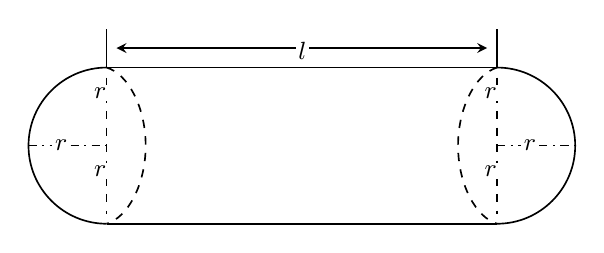
\begin{tikzpicture}[x=0.035cm, y=0.035cm, >=stealth, semithick, font=\small]

  % ===== 半球轮廓（上、下半弧，实线） =====
  \draw (0,56.67) .. controls (-15.60,56.67) and (-28.34,43.94) .. (-28.34,28.34)
        .. controls (-28.34,12.74) and (-15.60,0) .. (0,0);
  \draw (141.68,56.67) .. controls (157.28,56.67) and (170.01,43.94) .. (170.01,28.34)
        .. controls (170.01,12.74) and (157.28,0) .. (141.68,0);

  % ===== 圆柱母线（实线） =====
  \draw (0,56.67) -- (141.68,56.67);
  \draw (0,0) -- (141.68,0);

  % ===== 端面的内侧半椭圆与竖直直径（虚线） =====
  \draw[dashed] (0,56.67) .. controls (7.79,54.36) and (14.17,42.27) .. (14.17,28.34)
        .. controls (14.17,14.41) and (7.79,2.31) .. (0,0);
  \draw[dashed] (141.68,56.67) .. controls (133.89,54.36) and (127.51,42.27) .. (127.51,28.34)
        .. controls (127.51,14.41) and (133.89,2.31) .. (141.68,0);
  \draw[dashed] (0,52.98) -- (0,3.70);
  \draw[dashed] (141.68,52.98) -- (141.68,3.70);

  % ===== 半径标注线（点划线，照原页） =====
  \draw[dash dot] (-28.34,28.34) -- (0,28.34);
  \draw[dash dot] (141.68,28.34) -- (170.01,28.34);

  % ===== l 的双箭头 =====
  \draw[<->] (3.58,63.76) -- (138.09,63.76);
  \draw (0,56.67) -- (0,70.84);
  \draw (141.68,56.67) -- (141.68,70.84);
  \node[fill=white, inner sep=1pt] at (71.00,62.63) {$l$};

  % ===== r 标注（每端三条：竖直半径的上、下两段与朝外的水平半径） =====
  % 原页在标注处把虚线/点划线断开，本图用白底节点遮住线条，效果相同。
  \node[fill=white, inner sep=1pt] at (-2.30,47.38) {$r$};
  \node[fill=white, inner sep=1pt] at (139.38,47.38) {$r$};
  \node[fill=white, inner sep=1pt] at (-2.30,19.08) {$r$};
  \node[fill=white, inner sep=1pt] at (139.38,19.08) {$r$};
  \node[fill=white, inner sep=1pt] at (-16.50,28.58) {$r$};
  \node[fill=white, inner sep=1pt] at (153.58,28.58) {$r$};
\end{tikzpicture}
